\documentclass[11pt,a4paper,titlepage]{article}
\usepackage[brazil]{babel}
\usepackage[utf8]{inputenc}
\usepackage[T1]{fontenc}

\newcommand{\titulo}{\textit{Relatório IV - Unidade de Multiplicação}}

\newcommand{\cabecalho}{\textit{Relatório IV}}

\usepackage{fancyhdr}
\usepackage{indentfirst}
\usepackage{setspace}
\usepackage{graphicx,url}
\usepackage[section]{placeins}
%\usepackage{color,colortbl}
\usepackage{amsmath}
\usepackage{amssymb}
\usepackage{amsthm}
\usepackage{wrapfig}
\usepackage{times}
\usepackage{hyphenat}
\usepackage{ae}
\usepackage{algorithm}
\usepackage[sort,numbers]{natbib}
%package to insert codes
\usepackage{listings}
\usepackage{mips}
\usepackage{tabularx}
\usepackage{makecell}
%appendix
\usepackage[titletoc,toc,page]{appendix}
\renewcommand{\appendixtocname}{Apêndices}
\renewcommand{\appendixpagename}{Apêndices}

% the following is needed for syntax highlighting
\usepackage{color}

\definecolor{dkgreen}{rgb}{0,0.6,0}
\definecolor{gray}{rgb}{0.5,0.5,0.5}
\definecolor{mauve}{rgb}{0.58,0,0.82}

\lstset{ %código assembly
  language=[mips]Assembler,       % the language of the code
  basicstyle=\footnotesize,       % the size of the fonts that are used for the code
  numbers=left,                   % where to put the line-numbers
  numberstyle=\tiny\color{gray},  % the style that is used for the line-numbers
  stepnumber=1,                   % the step between two line-numbers. If it's 1, each line 
                                  % will be numbered
  numbersep=5pt,                  % how far the line-numbers are from the code
  backgroundcolor=\color{white},  % choose the background color. You must add \usepackage{color}
  showspaces=false,               % show spaces adding particular underscores
  showstringspaces=false,         % underline spaces within strings
  showtabs=false,                 % show tabs within strings adding particular underscores
  frame=single,                   % adds a frame around the code
  rulecolor=\color{black},        % if not set, the frame-color may be changed on line-breaks within not-black text (e.g. commens (green here))
  tabsize=4,                      % sets default tabsize to 2 spaces
  captionpos=b,                   % sets the caption-position to bottom
  breaklines=true,                % sets automatic line breaking
  breakatwhitespace=false,        % sets if automatic breaks should only happen at whitespace
  title=\lstname,                 % show the filename of files included with \lstinputlisting;
                                  % also try caption instead of title
  keywordstyle=\color{blue},          % keyword style
  commentstyle=\color{dkgreen},       % comment style
  stringstyle=\color{mauve},         % string literal style
  escapeinside={\%*}{*)},            % if you want to add a comment within your code
  morekeywords={*,...}               % if you want to add more keywords to the set
}
\usepackage{xcolor}
\definecolor{vgreen}{RGB}{104,180,104}
\definecolor{vblue}{RGB}{49,49,255}
\definecolor{vorange}{RGB}{255,143,102}
%mostrar código do verilog
\lstdefinestyle{verilog-style}
{
    language=Verilog,
    basicstyle=\small\ttfamily,
    keywordstyle=\color{vblue},
    identifierstyle=\color{black},
    commentstyle=\color{vgreen},
    numbers=left,
    numberstyle=\tiny\color{black},
    numbersep=10pt,
    tabsize=8,
    moredelim=*[s][\colorIndex]{[}{]},
    literate=*{:}{:}1
}

\makeatletter
\newcommand*\@lbracket{[}
\newcommand*\@rbracket{]}
\newcommand*\@colon{:}
\newcommand*\colorIndex{%
    \edef\@temp{\the\lst@token}%
    \ifx\@temp\@lbracket \color{black}%
    \else\ifx\@temp\@rbracket \color{black}%
    \else\ifx\@temp\@colon \color{black}%
    \else \color{vorange}%
    \fi\fi\fi
}
\makeatother

\usepackage{trace}

% Criar figura dividida em subfiguras
\usepackage{subfigure}

\usepackage{subfig}
\usepackage{ae}
\usepackage{aecompl}

\usepackage{multirow}
%\usepackage{epstopdf}

\pagestyle{fancy}

\setlength{\evensidemargin}{0.0in}
\setlength{\oddsidemargin}{0.0in}
\setlength{\textwidth}{6.6in}
\setlength{\textheight}{1.06\textheight}

\lhead{}
\chead{}
\rhead{\footnotesize{\textsc{\cabecalho}}}
\lfoot{\footnotesize{Iuri Silva Castro, João Mateus de Freitas Veneroso, Ricardo Pagoto Marinho}}
\cfoot{}
\rfoot{\footnotesize{\thepage}}
\setlength{\headwidth}{\textwidth}
\renewcommand{\headrulewidth}{0.4pt}
\renewcommand{\footrulewidth}{0.4pt}
\renewcommand{\baselinestretch}{0.90}

%\hyphenation{ ca-rac-te-ri-zan-do--se }

\begin{document}

\begin{titlepage}
\begin{center}

\begin{large}
Universidade Federal de Minas Gerais\\
Instituto de Ciências Exatas\\
Departamento de Ciência da Computação\\
\end{large}

\vspace{20mm}

\begin{Large}
DCC819 - Arquitetura de Computadores
\end{Large}

\vspace{20mm}

\begin{LARGE}
\titulo
\end{LARGE}


\vspace{30mm}

\begin{Large}
\begin{center}
Iuri Silva Castro\\ João Mateus de Freitas Veneroso\\ Ricardo Pagoto Marinho \\
\end{center}
\end{Large}


\vspace{60mm}

{\sc Belo Horizonte - MG}

{\sc \today}

%\vspace{10mm}
\end{center}
\end{titlepage}


\section{Descrição}\label{sec:desc}

Até a atual implementação o processador proposto não possuía instrução de multiplicação específica. Deseja-se agora implementar a instrução \textit{MUL}, que fará a multiplicação de dois registros de 16-bit, armazendo o resultado em dois registros \textit{HI} e \textit{LO}, ambos de 16-bit, sendo que o registro \textit{HI} mantém os 16-bit mais significativos e o registro \textit{LO} mantém os 16-bit menos significativos. A fim de melhorar o desempenho de tal instrução, um módulo (hardware) de multiplicação dedicado será implementado, não havendo alterações no funcionamento da ULA. Duas instruções \textit{GHI} e \textit{GLO} foram implementadas para fazer o armazenamento de tais registros no banco de registradores.

A implementação do módulo e das instruções são descritas nas seções seguintes. Textes e discussões são feitas ao final do trabalho.

\section{Implementação}

Inicialmente, propõe-se a implementação do módulo de multiplicação, que será paralelo a \textit{ULA}. O módulo recebe dois operandos de 16-bit e retorna o resultado em 32-bit. O diagrama pode ser visto na figura \ref{fig:mult}.

\begin{figure}[!h]
\centering
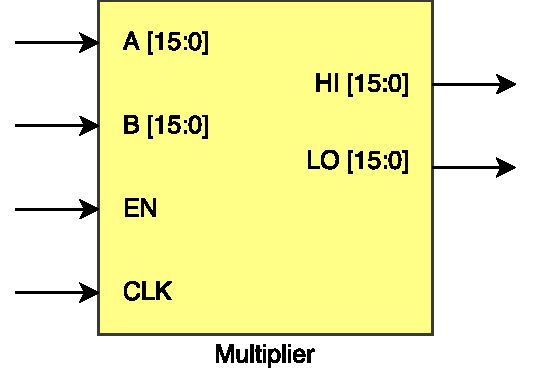
\includegraphics[scale=0.5]{images/Multiplier.pdf}
\caption{Módulo de multiplicação.}
\label{fig:mult}
\end{figure}

Os sinais de \textit{clock} (\textit{CLK}) e \textit{enable} (\textit{EN}) são utilizados para sincronizar e atualizar os valores dos registros \textit{HI} e \textit{LO}, que são mantidos dentro do módulo.

Com a adição de mais um módulo é necessário modificar o sistema de controle da máquina, para dar suporte as novas instruções e ao novo módulo. As instruções adicionadas foram:

\begin{itemize}
\item \textit{MUL -, opA, opB}: Multiplica o operador A com o B, o resultado é armazenado nos registros \textit{HI} e \textit{LO}, interno ao módulo;
\item \textit{GHI dest, -, -}: Acessa o registro \textit{HI} dentro do módulo de multiplicação e armazena no registrador \textit{dest} especificado;
\item \textit{GLO dest, -, -}: Acessa o registro \textit{LO} dentro do módulo de multiplicação e armazena no registrador \textit{dest} especificado.
\end{itemize}

A instrução de multiplicação não altera diretamente o banco de registradores, sendo necessário as duas instruções auxiliares. O diagrama do módulo de controle pode ser visto na figura \ref{fig:ctrl}.

\begin{figure}[!h]
\centering
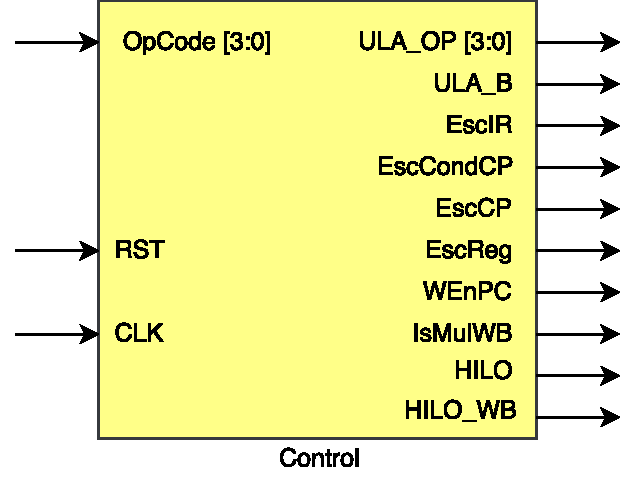
\includegraphics[scale=0.5]{images/Control.pdf}
\caption{Módulo de controle.}
\label{fig:ctrl}
\end{figure}

Os novos sinais \textit{IsMulWB}, \textit{HILO} e \textit{HILO-WB} foram adicionados para fazer o encaminhamento dos dados do multiplicador para o banco de registradores e indicar ao multiplicador que ele deve atualizar os registros \textit{HI} e \textit{LO}.

Com o módulo implementado e as atualizações feitas, parte-se parar a integração do sistema.

\section{Integração}

Com a adição do módulo de multiplicação, alterações são necessárias no encaminhamento dos dados para dentro e fora do módulo. Dois multiplexadores foram adicionados para fazer os encaminhamentos. A figura \ref{fig:impl} mostra como ficou o sistema.

\begin{figure}[!h]
\centering
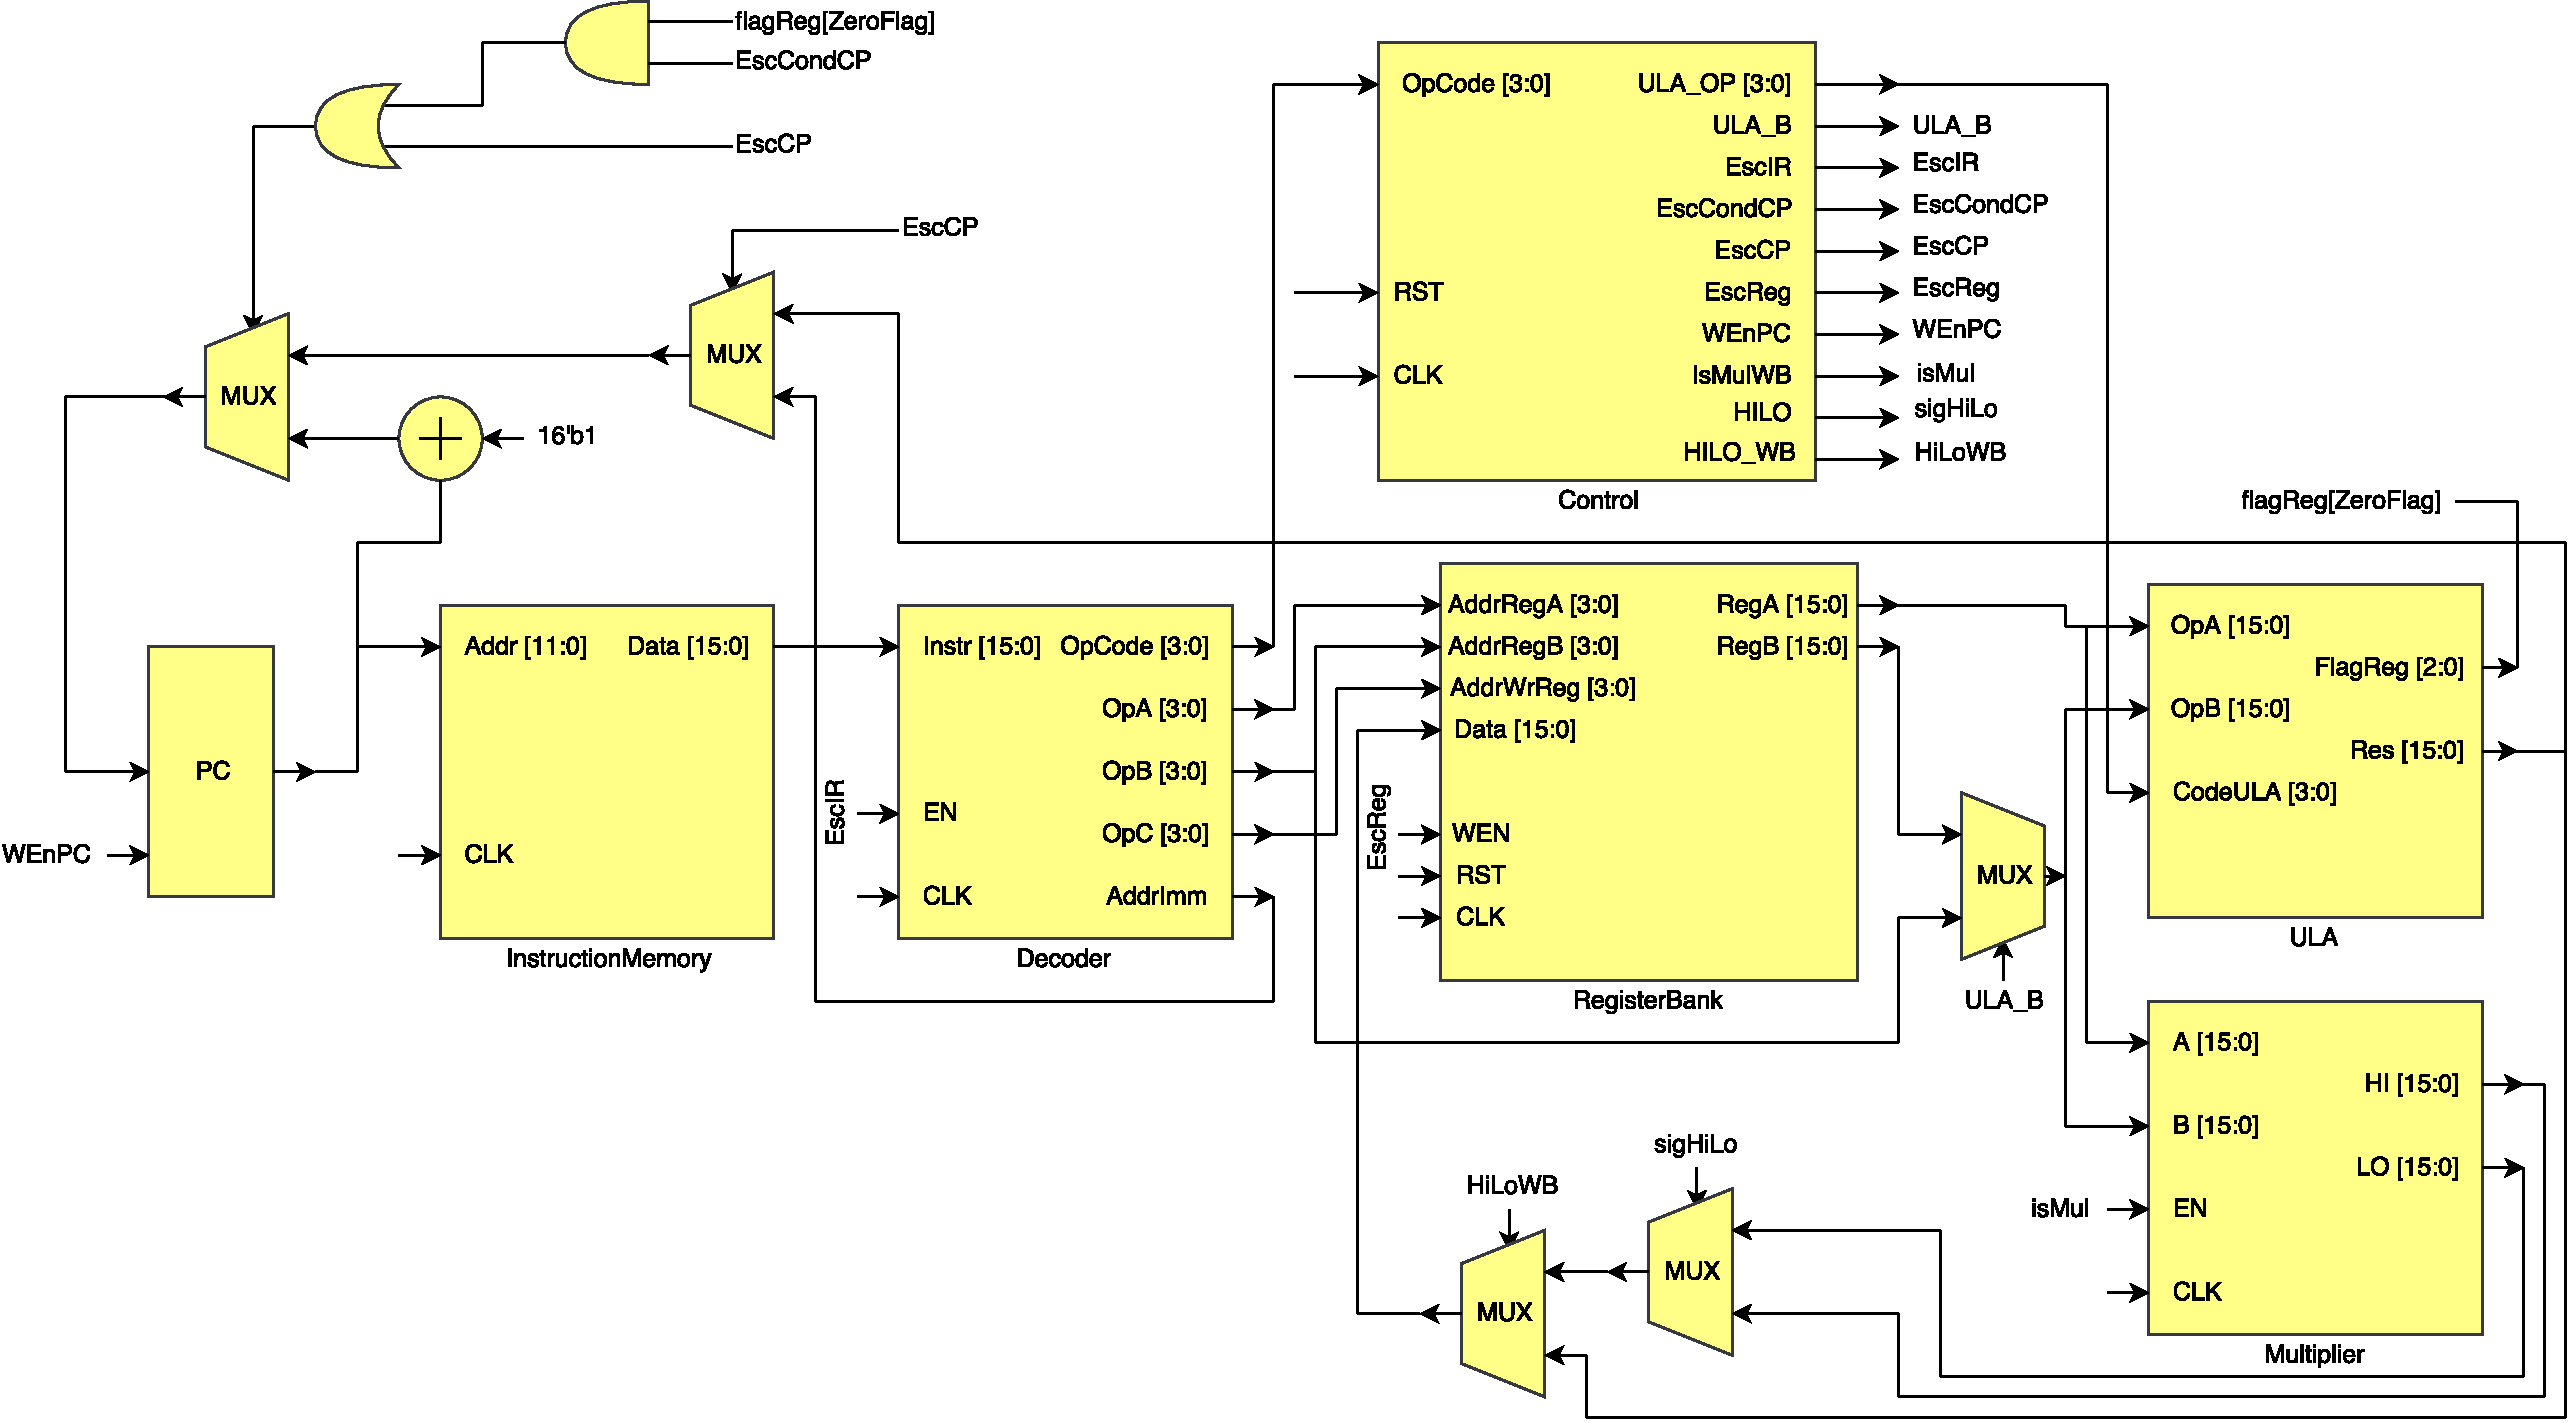
\includegraphics[scale=0.4]{images/Microprocessor.pdf}
\caption{Integração do sistema.}
\label{fig:impl}
\end{figure}

O sinal \textit{HILO} indica qual dos registradores da multiplicação será armazenado no banco de registradores, o sinal \textit{HILO-WB} indica o módulo que ele deve atualizar os registradores \textit{HI} e \textit{LO}, pois uma nova multiplicação foi executada e o sinal \textit{IsMulWB} indica se está trabalhando com dados da ULA ou do multiplicador.

\section{Simulação e Testes}

Para o teste de execução, preparou-se 4 multiplicações para serem simuladas no software ModelSim. No início da simulação, reinicia-se a máquina para zerar os valores dos registros e inicializar a máquina de estado do módulo de controle. Após a reinicialização da máquina, carrega-se os valores a serem multiplicados no banco de registradores diretamente, e defini-se as instruções de multiplicação e de armazenamento do resultados a nível de software, não utilizou-se, dessa vez, o arquivo para inicialização da memória de instruções. A figura \ref{fig:modelsim} mostra a saída da simulação. 

\begin{figure}[!h]
\centering
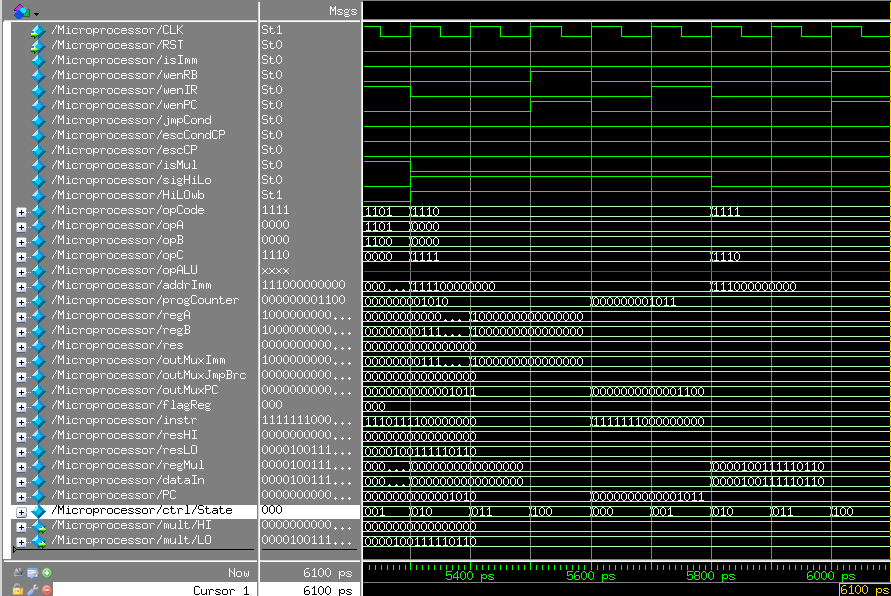
\includegraphics[scale=0.5]{images/sim.png}
\caption{Formas de onda de saída da simulação.}
\label{fig:modelsim}
\end{figure}

Os valores dos testes foram os seguintes:

\begin{itemize}
\item \textit{Teste 1}: 128 (Reg0) x 5 (Reg1); HI (Reg3) LO (Reg2)
\item \textit{Teste 2}: 65535 (Reg4) x 15 (Reg5); HI (Reg7) LO (Reg6)
\item \textit{Teste 3}: 500 (Reg8) x 500 (Reg9); HI (Reg11) LO (Reg10)
\item \textit{Teste 4}: 255 (Reg12) x 10 (Reg13); HI (Reg15) LO (Reg14)
\end{itemize}

O resultado no após a simulação pode ser observado no banco de registradores, conforme figura \ref{fig:res}.

\begin{figure}[!h]
\centering
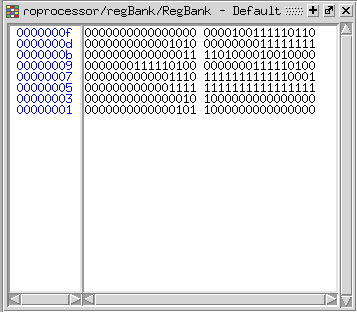
\includegraphics[scale=0.5]{images/res.png}
\caption{Resultado no banco de registradores.}
\label{fig:res}
\end{figure}


\section{Discussões}

A instrução \textit{SLT reg-reg}, adicionada no trabalho passado para auxiliar na ordenação dos registros, foi removida, pois o tamanho de instruções atual só permite a indexação de 16 opcodes, e não haveria espaço para adicionar as 3 novas instruções necessárias.

A instrução de multiplicação implementada trabalha apenas com números inteiros positivos.

\bibliographystyle{unsrt}
\addcontentsline{toc}{section}{Referências}
%\bibliography{references}

\nocite{*}


\end{document}

